\documentclass[a4paper,10pt]{article}

\usepackage[utf8x]{inputenc}
\usepackage[slovene]{babel}
\usepackage{amsmath}
\usepackage{amsfonts}
\usepackage{relsize}
\usepackage[smaller]{acronym}
\usepackage{graphicx}
\usepackage{subfigure}
\usepackage{cite}
\usepackage{url}
\usepackage{hyperref}
\usepackage{color}
\usepackage[version=3]{mhchem}
\usepackage{wrapfig}

%opening
\title{Hidrodinamske nestabilnosti}

\renewcommand{\vec}{\mathbf}
\newcommand{\eps}{\varepsilon}
\renewcommand{\phi}{\varphi}
\renewcommand{\theta}{\vartheta}

\newcommand{\norm}[1]{\lVert #1 \rVert}

\newcommand{\rt}{(\vec r, t)}

\begin{document}
\begin{center}

\includegraphics[width=6cm]{../logo_fmf_uni-lj_sl}\\[0.5cm]
Oddelek za fiziko \\[2cm]
{ \large Seminar -- 1. letnik, II. stopnja } \\[1cm]
{ \huge \bf Hidrodinamske Nestabilnosti}\\[2cm]
{\large Avtor: Miha \v Can\v cula}\\[0.6cm]
{\large Mentor: prof. dr. Alojz Kodre} \\[0.6cm]
{\large Ljubljana, marec 2012}
\end{center}
\vfill

\begin{abstract}

\end{abstract}

\newpage

\tableofcontents

\section{Uvod}

\section{Stabilnost}

O nestabilnosti govorimo, ko infinitezimalno majhna sprememba trenutnega stanja lahko povzro"ci ve"cjo, merljivo razliko po nekem kon"cnem "casu~\cite{drazin}. 

Tak"sna definicija je precej splo"sna, zato jo za potrebe seminarja raje definiramo o"zje in bolj eksaktno: Imejmo sistem, katerega "casovno spreminjanje lahko z eno ali ve"c diferencialnimi ena"cbami, ki imajo dolo"ceno simetrijo. Z nastavkom, ki upo"steva to simetrijo, lahko dobimo re"sitev ena"cb. Stabilnost se poka"ze, ko temu nastavku dodamo majhno motnjo, ki ne upo"steva simetrije. Stabilni sistem se bo vrnil v simetri"cno stanje, medtem ko pri nestabilnem pride do zloma simetrije. 

Primer nestabilnega pojava je svin"cnik, postavljen na konico. Ena"cba, ki opisuje njegovo gibanje, je simetri"cna glede na rotacijo okrog osi svin"cnika. Zato lahko najdemo re"sitev z enako simetrijo, to je pokon"cna lega. "Ce pa svin"cnih le malo izmaknemo iz simetri"cne lege, bo padel in kon"cal v stanju brez rotacijske simetrije. 

\section{Hidrodinamika}

\subsection{Navier-Stokesova ena"cba}

Tok nestisljive teko"cine z gostoto $\rho$ in viskoznostjo $\mu$ se podreja Navier-Stokesovi ena"cbi in ohranitvi mase

\begin{align}
 \label{eq:ns-enacba}
\frac{\partial \vec u}{\partial t} + \vec u \cdot \nabla \vec u &= -\frac{1}{\rho}\nabla p + \mu \Delta \vec u \\
\nabla \vec u &= 0
\end{align}

Kot obi"cajno pri re"sevanju ena"cb si jo najprej poenostavimo tako, da preidemo na brezdimenzijske spremenljivke in "cimbolj minimiziramo "stevilo parametrov. Izberimo si meri za dol"zino $x_0$ in hitrost $v_0$. "Ce uvedemo "se brezdimenzijsko Reynoldsovo "stevilo $R=v_0 x_0 / \mu$, lahko ena"cbo zapi"semo za brezdimenzijski spremenljivki $U$ in $P$. 

\begin{align}
 \label{eq:ns-brezdim}
\frac{\partial \vec U}{\partial t} + \vec U \cdot \nabla \vec U &= -\nabla P + R^{-1} \Delta \vec U \\
\nabla \vec U &= 0
\end{align}

\subsection{Lineariziran problem}

Stabilnost hidrodinamskega sistema lahko "studiramo tako, da najprej najdemo osnovno re"sitev, ki ji v hidrodinamiki re"cemo \emph{osnovni tok}. Ta re"sitev je lahko podana analiti"cno ali numeri"cno, vsekakor pa se podreja Navier-Stokesovi ena"cbi. Podamo jo kot polje hitrosti $\vec U(\vec r, t)$ in tlaka $P(\vec x, t)$. 

Nato osnovnem toku dodamo motnjo, tako da dobimo \emph{skupni tok}, zopet podan s hitrostjo $\vec u = \vec U + \vec u'$ in tlakom $p = P + p'$. Tudi za skupni tok mora veljati N-S ena"cba, iz "cesar lahko izpeljemo ena"cbo za motnjo $u'$ in $p'$. 

Stabilnost sistema pomeni, da vse motnje, ki so na za"cetku majhne, ostanejo majhne tudi ob poljubnem "casu. Nasprotno, sistem je nestabilen, "ce vsaj ena motnja po nekem "casu preneha biti majhna. Za matemati"cni opis moramo to difincijo formalizirati in dolo"citi mero za velikost motnje. 

Tok je \emph{stabilen}, "ce za vsak $\eps > 0$ obstaja $\delta(\eps) > 0$, tako da za 
\begin{equation}
 \norm{ u'(\vec r, 0) }, \; \norm{ p'(\vec r, 0) } < \delta
\end{equation}
velja
\begin{equation}
 \norm{ u'\rt }, \; \norm{ p'\rt } < \eps \;\;\;\; \forall t > 0
\end{equation}

"Ce je tok stabilen in velja
\begin{equation}
 \norm{u'\rt}, \; \norm{p'\rt} \xrightarrow[t\to\infty]{} 0
\end{equation}
torej se motnja s "casom manj"sa, je tok \emph{asimptoti"cno stabilen}. V teoriji dinami"cnih sistemov asimptoti"cno stabilni re"sitvi re"cemo tudi atraktor. 

Ker nas zanimajo le majhne motnje, lahko v ena"cbi zanemarimo vse "clene kjer motnja nastopa v drugem ali vi"sjih redih. Na ta na"cin sistem zreduciramo na linearno diferecialno ena"cbo 

\begin{align}
 \label{eq:ns-linearna}
\frac{\partial \vec u'}{\partial t} + \vec U \cdot \nabla \vec u' + \vec u' \cdot \nabla \vec U &= -\nabla p' + R^{-1}\Delta u' \\
\label{eq:nestisljivost-linearna}
\nabla \cdot \vec u' &= 0
\end{align}

"Ce je osnovni tok stacionaren, so koeficienti v linearnem sistemu ena"cb konstantni, zato lo"cimo spremenljivki $\vec r$ in $t$, splo"sno re"sitev pa zapi"semo kot linearno kombinacijo normalnih na"cinov 

\begin{align}
 \vec u'\rt &= \sum e^{s_i t} \vec u_i(\vec r) \\
 p'\rt &= \sum e^{s_i t} p_i(\vec r)
\end{align}

Hitro lahko vidimo, da bo tok nestabilen, "ce ima vsaj ena lastna vrednosti $s_i$ realni del ve"cji od 1, v nasprotnem primeru pa bo stabilen. Problem stabilnosti sistema lahko torej prevedemo na iskanje lastnih vrednosti matrike. 

\section{Tanki filmi}

Hidrodinamsko nestabilnost lahko opazujemo pri polzenju teko"cine po klan"cini~\cite{kondic}. 

\begin{figure}[h]
\centering
 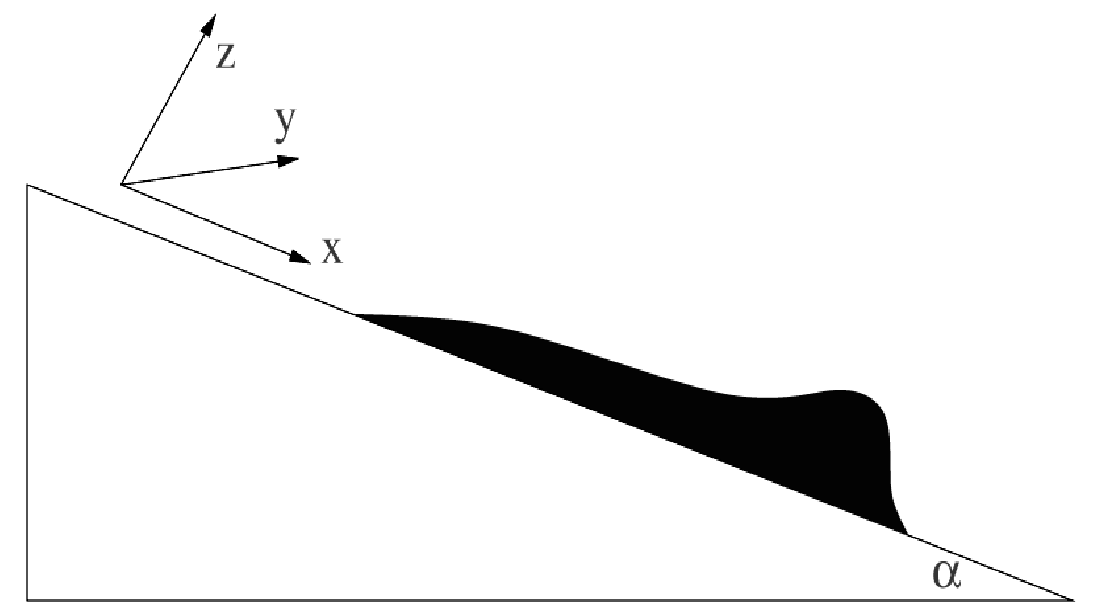
\includegraphics[width=.8\textwidth]{./Slike/film-skica}
\caption{Skica teko"cine v dveh dimenzijah. Viden je greben tik za fronto teko"cine in pa zo"zitev dale"c za fronto, ki je pri ra"cunih ne bomo upo"stevali}
\label{fig:film-skica}
\end{figure}

\subsection{Ena"cbe}

"Ce privzamemo nestisljivost teko"cine $\nabla \cdot \vec u = 0$, se Navier-Stokesova ena"cba poenostavi v 

\begin{align}
 \label{eq:ns-film}
 \frac{\partial \vec u}{\partial t} + (\nabla \cdot \vec u) &= -\frac{1}{\rho}\nabla p + \frac{\mu}{\rho}\nabla^2 \vec u + g (\sin \alpha \vec i - \cos \alpha \vec k)
\end{align}

kjer je $\vec u$ hitrost teko"cine, $\rho$ njena gostota in $\mu$ viskoznost. "Clena z $g$ sta dinami"cna in stati"cna komponenta sile te"ze. Pomembni so tudi robni pogoji, obi"cajno se izbere slede"ce:

\begin{itemize}
 \item Na meji med teko"cino in klancem teko"cina ne drsi, torej je tam $\vec u = 0$. 
 \item Na meji med teko"cino in zrakom ima tlak nezveznost, ki jo sorazmerja povr"sinski napetosti in ukrivljenosti meje $\kappa$. 
\end{itemize}

Ker obravnavamo tanke filme, lahko privzamemo, da je debelina $h$ manj"sa od katerekoli dol"zinske skale v ravnini. S tem privzetkom lahko ena"cbo (\ref{eq:ns-film}) poenostavimo v ena"cbo za $h$. 

\begin{align}
 \frac{\partial h}{\partial t} = -\frac{1}{3\mu}\nabla \cdot \left[ \gamma h^3 \nabla \nabla^2 h - \rho g h^3 \nabla h \cos \alpha + \rho g h^2 \sin \alpha \vec i \right]
\end{align}

\subsubsection{Brezdimenzijska oblika}

\subsection{Nestabilnost}

\begin{figure}[h]
\centering
 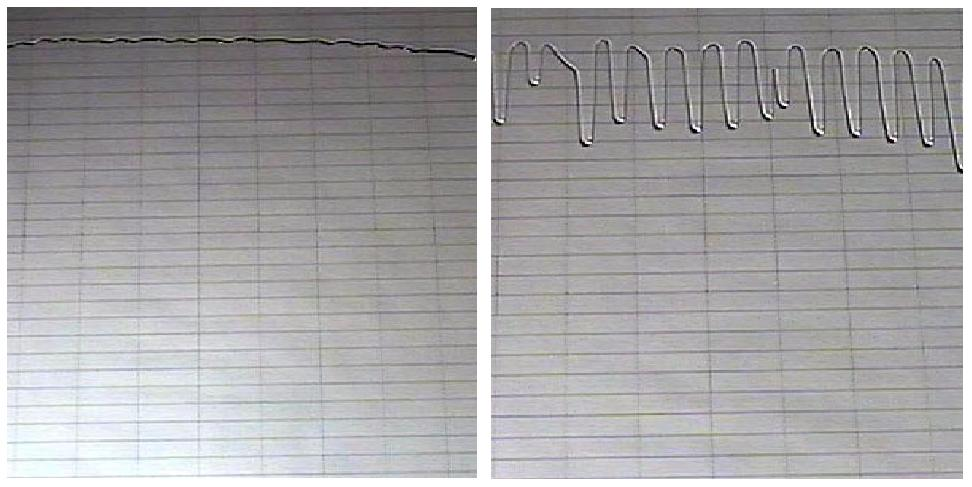
\includegraphics[width=.9\textwidth]{./Slike/film-slika}
\caption{Polzenje tanke plasti teko"cine po nagnjeni povr"sini. Majhne motnje v obliki fronte (levo) hitro prerastejo v vzorec, ki ni niti pribli"zno enakomeren (desno). Vir: \cite{kondic}}
\label{fig:film-neenakomernost}
\end{figure}


\section{Milni mehur"cki}

Milni mehur"cki so stabilni na majhne motnje zaradi povr"sinske napetosti teko"cine. "Ce pa mehur"cek predremo v eni to"cki, ustvarimo rob, kjer povr"sinska napetost ni uravnote"zena, zato se rob za"cne umikati. Ker je opna obi"cajno zelo tanka, 
je ukrivljenost na robu velika, zato fronta napreduje zelo hitro~\cite{diploma}. To napredovanje je pri mehur"ckih tako hitro, da s prostim o"cesom fronte sploh ne opazimo, ampak se nam zdi, da celoten mehur"cek razpade naenkrat. 
 
\begin{figure}[h]
 \centering
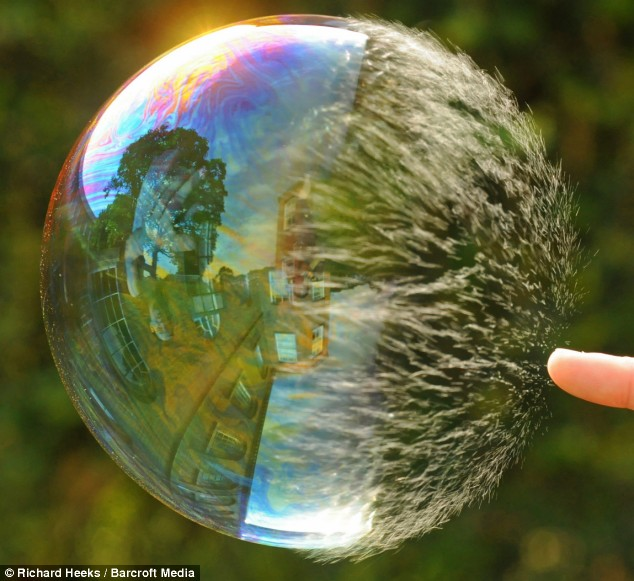
\includegraphics[width=.8\textwidth]{./Slike/bubble-3}
\caption{Razpad milnega mehir"cka~\cite{slike-mehurcek}. Kapljice na desni strani niso posejane enakomerno, ampak so vidni pasovi ve"cje in manj"se gostote. }
\label{fig:mehurcek-3}
\end{figure}

\subsection{Ena"cbe}

Podobno kot pri tankem filmu lahko tudi za opno predpostavimo, da je tanka, njeno debelino pa ozna"cimo s $h = h(x,t)$. Opna ima translacijsko simetrijo v smeri $y$, zato na za"cetku predpostavimo, da imajo tak"sno simetrijo tudi $h$ ter gostota in tlak teko"cine. 

\subsection{Nestabilnost}

\section{Curki}

Na nestabilnosti pogosto naletimo tudi pri "studiju curkov teko"cin~\cite{eggers}. 


\section{Zaklju"cek}

\begin{thebibliography}{3}
  \bibitem{diploma} S. "Copar, Numeri"cna analiza nestabilnosti na robu teko"cinske opne, Diplomsko delo (2009)
  \bibitem{kondic} L. Kondic, SIAM Review \textbf{45}, 95 (2003)
  \bibitem{eggers} J. Eggers in E. Villermaux, Rep. Prog. Phys. \textbf{71}, 036601 (2008)
  \bibitem{drazin} P. G. Drazin, \textit{Introduction to hydrodynamic stability}, Cambridge University Press (2002)
  \bibitem{slike-mehurcek} \url{http://www.dailymail.co.uk/sciencetech/article-1199149/Super-slow-motion-pictures-soap-bubble-bursting-stunning-detail.html} (23. 1. 2012)
\end{thebibliography}


\end{document}
